\documentclass[]{template}

% En-tête
\renewcommand{\headrulewidth}{0.1pt}
\fancyhead[C]{} 
\fancyhead[L]{\rightmark}
\fancyhead[R]{\thepage}

% Pied de page
\newcommand{\tablemat}{~}
\renewcommand{\tablemat}{\tableofcontents}
\renewcommand{\footrulewidth}{0.1pt}
\fancyfoot[C]{} %\textbf{\thepage} 
\fancyfoot[L]{}
\fancyfoot[R]{Source coding, data compression and
channel coding}

\begin{document}

\begin{guardpage}
    \academicyear{2024-2025}
    %\guardimage{de}{0.8}
    \addtitle{ELEN0060-2: Project 2}{Source coding, data compression and
    channel coding}
    \begin{authors}{0.18}
        \addauthor{Pierre}{Lorenzen}{S203724}
        \addauthor{Abdelilah}{Khaliphi}{S204896}
    \end{authors}

\end{guardpage}

\newpage
\tablemat
\newpage

\section{Implementation}

    \subsection{Question 1}
        In the implementation for this question, we first define a node class to facilitate the creation and management of the binary tree used in the Huffman coding algorithm.\\
        
        \noindent
        Secondly, iteratively, we sort the nodes based on their probabilities at each iteration, and we merge the two lowest probabilities. This node created
        by the merge of the two lowest probabilities ones is then added to the tree with a probability equal to the sum of the two lowest probabilities. 
        The children nodes are the two nodes that were merged. The process is repeated until we have a single node left, which is the root of the tree. \\

        \noindent
        Tirdly, we generate the codes for each symbol by traversing the tree. We start at the root and assign a '0' code to the left child and a '1' code to
        the right child. We continue this process recursively until we reach a leaf node, at which point we store the generated code for that symbol.\\

        \noindent
        Finally, we reorder the symbols to be consistent with the order provided at the input of the function.\\

        \noindent
        To extend the Huffman code generation to any alphabet size $q$, we can modify the algorithm to merge the q lowest-probabilities
        nodes at each step and so build a q-ary tree, where each node has up to $q$ children.\\
        
        \noindent
        To implement this with a number of input symbols $n$ and output alphabet size of $q \geq 2$, we can
        
        \begin{enumerate}
            \item Take the $n$ symbols with their probabilities
            \item Add Dummy Symbols: If $(n-1) \; mod \; (q-1) \neq  0$, add dummy symbols of probability 0 so that:
            $(n' - 1) \; mod \; (q-1)=0$
            
            where n' is the total number of symbols (real + dummy).
            \item Maintain nodes sorted by probability.  
            \item Merge q smallest-nodes.
            \item Repeat until only one node is left.
            \item Label the edges with 0,1,\ldots,q-1.
        \end{enumerate}
        
    \subsection{Question 2}

    Initially, the dictionary is established with an empty string mapped to index 0. 
    The algorithm then iterates through each character of the input sequence, progressively building phrases.
    For each iteration, it combines the current phrase with the next character from the input to form 
    a new candidate phrase. 
    If this new phrase is not already present in the dictionary, the algorithm performs two operations:

    \begin{itemize}
        \item It appends a tuple containing the index of the current phrase (as found in the dictionary) 
            and the character that triggered the creation of the new phrase to the encoded\_sequence.
        \item It then adds the new phrase to the dictionary with a unique incremental index.
    \end{itemize}

    \noindent
    The current phrase is reset after each dictionary insertion, allowing the process to restart and 
    construct new phrases from subsequent characters. If the new phrase is already present in the dictionary,
    the algorithm continues extending it until it encounters a unique phrase.\\

    \noindent
    After processing the entire sequence, any remaining unprocessed phrase is handled explicitly 
    by adding a final tuple to the encoded sequence.\\

    \noindent
    Applying this algorithm to the given example sequence "ababcbababaaaaaaa", results in constructing 
    a dictionary that maps substrings to indices, and produces an encoded sequence consisting of tuples 
    representing dictionary indices paired with subsequent characters.\\

    \noindent
    This approach effectively exploits repeating patterns within data, significantly reducing the 
    size required for storage or transmission, making it a practical and efficient method in data 
    compression scenarios.

    \subsection{Question 3}

    As explained in the theoretical course, the Lempel-Ziv algorithms can be compared on several aspects. 
    These aspects are the dictionary construction, the parsing of the input data, 
    the encoding, the dictionary address size, the adaptivity of the algorithm, 
    the efficiency, and the on-line capability.
    See table \ref{tab:basic_vs_online} for a comparison of the two algorithms.\\
    \begin{table}[ht]
        \centering
        \setlength{\tabcolsep}{6pt}
        \begin{tabular}{|p{3cm}|p{5cm}|p{5cm}|}
            \hline
            \multicolumn{1}{|c|}{Aspect} & \multicolumn{1}{c|}{Basic Lempel-Ziv} & \multicolumn{1}{c|}{On-line Lempel-Ziv} \\ \hline
            Dictionary construction      & Grows incrementally by adding new words & Same as basic \\ \hline
            Parsing                      & Greedy: find the longest prefix in dictionary & Same as basic \\ \hline
            Encoding                     & Tuple (address of prefix, next symbol) & Same as basic but address is encoded dynamically \\ \hline
            Dictionary address size      & Fixed-size = $2^n$\newline (where n is number of bits) & Variable-length based on current dictionary size \\ \hline
            Adaptivity                   & No adaptation based on dictionary & Fewer bits used at early stages \\ \hline
            Efficiency                   & Good compression with large dictionary & More efficient in early stages due to shorter addresses \\ \hline
            On-line capability           & No & Yes, can transmit as text is read \\ \hline
        \end{tabular}
        \caption{Comparison of Basic Lempel-Ziv and On-line Lempel-Ziv}\label{tab:basic_vs_online}
    \end{table}

    \noindent
    Base on this comparison, we can conclude that the advantages of the basic Lempel-Ziv algorithm are that the compression on large dictionary is 
    more efficient than the on-line Lempel-Ziv algorithm, and that the dictionary address size is fixed. 
    The backwards of this version is that it is not adaptive, and it is not on-line.\\

    \noindent
    The advantages of the on-line Lempel-Ziv algorithm are that it is adaptive, on small and medium dictionary size the efficiency is better due to the shorter addresses, and it is on-line. The backwards of this version is that the compression
    on large dictionary is less efficient than the basic Lempel-Ziv algorithm, and that the dictionary address size is variable.\\

    \subsection{Question 4}

    To decode a LZ77 encoded text, we need first to reset the basis. The encoded text is a 
    sequence of triples (Offset, Length, NextChar). 
    To decode a full sequence of triple, the same logic is applied to each triple in the sequence.\\

    \noindent
    Firstly, \textbf{if the offset is 0 and the length is 0}, then the next
    character can be appended to the output string.\\

    \noindent
    Secondly, \textbf{if the offset is not 0 and the length is not 0}, then we 
    need to move back by the specified offset in the output string and copy 
    the specified length of characters from the output string to the output string.
    After that we can add the next character to the output string.\\

    \noindent
    This process is repeated until we have decoded the entire sequence of triples.\\

    \noindent
    \textbf{Example:}\\
    \noindent
    If the encoded text is (0, 0, 'a'),
    (0, 0, 'b'),
    (0, 0, 'r'),
    (3, 1, 'c'),
    (5, 1, 'd'),
    (7, 4, 'd'). The decoding algorithm will run like seen in the table \ref{tab:decoding}: 

    \begin{table}[ht]
        \centering
        \begin{tabular}{|c|c|c|}
        \hline
        Triple      & Current output string & Afterwards output string \\ \hline
        (0, 0, 'a') & " "                   & "a"                      \\ \hline
        (0, 0, 'b') & "a"                   & "ab"                     \\ \hline
        (0, 0, 'r') & "ab"                  & "abr"                    \\ \hline
        (3, 1, 'c') & "\color{blue}{a}\color{black}{br}"                 & "abr\color{blue}{a}\color{black}c"                  \\ \hline
        (5, 1, 'd') & "\color{blue}{a}\color{black}brac"               & "abrac\color{blue}{a}\color{black}d"                \\ \hline
        (7, 4, 'd') & "\color{blue}abra\color{black}cad"             & "abracad\color{blue}abra\color{black}d"           \\ \hline
        \end{tabular}
        \caption{Decoding of the encoded text}\label{tab:decoding}
    \end{table}

\section{Source coding and reversible (lossless) data compression}

    \subsection{Question 5}

    \noindent
    After having estimated the marginal probabilities of all the 27 symbols, determine the Huffman codes for each symbol, 
    and encoded the English text. You can find the results in the table \ref{tab:huffman}.\\

    \begin{table}[ht]
        \centering
        \begin{tabular}{|c|c|c|}
        \hline
                                     & Total encoded text length & Compression rate   \\ \hline
        Huffman coding               & 239,008                   & 1.9496585888338465 \\ \hline
        \end{tabular}
        \caption{Results of the Huffman coding}\label{tab:huffman}
    \end{table}

    \subsection{Question 6}

    The average length for our Huffman code is $4.10328$ bits. \\

    \noindent
    Let's compare this value with the empirical average length.
    We can see that the empirical average length is $4.10328$. So,\\
    \[
        empirical_{avg} = 4.10328 = expected_{avg}
    \]


    \noindent
    The theoretical bounds of a Huffman code are related to how closely its average codeword 
    length approximates the entropy of the source.
    \[
        \frac{H(S)}{\log \; q} \leq \overline{n} < \frac{H(S)}{\log \; q} + 1 
    \]

    \noindent
    This means that the probabilities used to build the Huffman code match exactly the observed frequencies in the text.
    That was expected because the Huffman code is built based on the frequencies of the symbols in the text.
    This means that our algorithm works well.

    \noindent
    By knowing that the entropy in this case is \[H(S) = 4.06223\] and 
    with $q = 2$ because the size of the alphabet is 2 (the Huffman tree is a binary tree), we can calculate the bounds of the average codeword length:
    \begin{align*}
        \frac{4.06223}{\log 2} &\leq \overline{n} < \frac{4.06223}{\log 2} + 1 \\
        4.06223 &\leq \overline{n} < 5.06223
    \end{align*}
    
    \noindent
    We can see that the expected average length is $4.10328$ which is between the bounds $4.06223$ and $5.06223$.
    The value of the expected average length tells us that the Huffman code is near-optimal.

    \subsection{Question 7}

    The empirical average code length evolution with text length is shown in the figure 
    \ref{fig:evolution_avg_code_length}.\\
    
    \begin{figure}[ht]
        \centering
        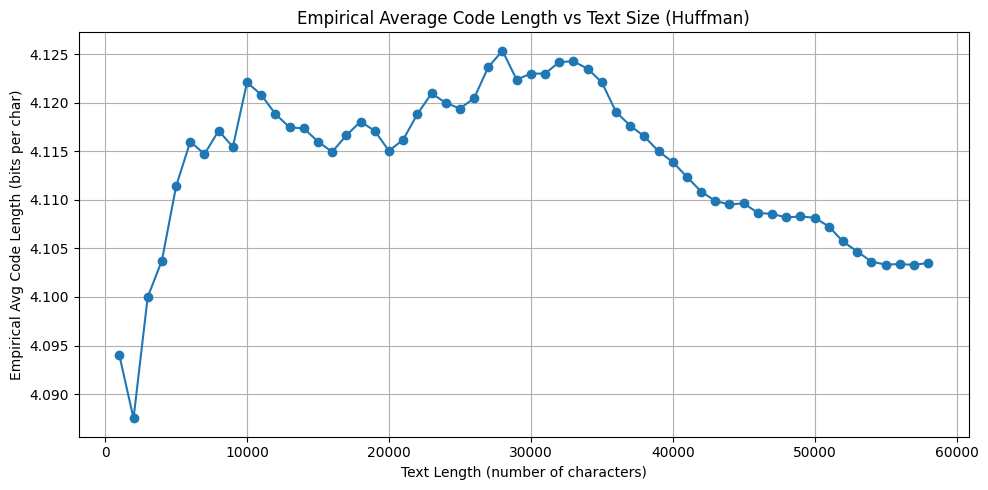
\includegraphics[width=1\textwidth]{Images/evolution_avg_code_length.png}
        \caption{Empirical average code length evolution with text length}\label{fig:evolution_avg_code_length}
    \end{figure}

    \noindent
    We can see that the empirical average code length is decreasing with the text length.
    This means that the Huffman code is getting better as the text length is increasing.
    We can also see that the empirical average code length is growing exponentially until we reach the 10,000 characters.
    This demonstrates that the Huffman code is not optimal for short texts.

    \subsection{Question 8}

    You can find the results in the table \ref{tab:online_lz77}.

    \begin{table}[ht]
        \centering
        \begin{tabular}{|c|c|c|}
        \hline
                                     & Total encoded text length & Compression rate   \\ \hline
        on-line Lempel-Ziv algorithm & 233,396                   & 1.9965380726319217 \\ \hline
        \end{tabular}
        \caption{Results of the on-line Lempel-Ziv algorithm}\label{tab:online_lz77}
    \end{table}

    \subsection{Question 9}

    You can find the results in the table \ref{tab:lz77_window_size_7}.

    \begin{table}[ht]
        \centering
        \begin{tabular}{|c|c|c|}
        \hline
                                     & Total encoded text length & Compression rate   \\ \hline
        LZ77 window size of 7        & 441,364                   & 1.0557816224250278 \\ \hline
        \end{tabular}
        \caption{Results of the LZ77 algorithm with a window size of 7 characters}\label{tab:lz77_window_size_7}
    \end{table}

    \subsection{Question 10}

    One straightforward method for combining LZ77 and Huffman coding involves a two-stage process. 
    First, the input text is compressed using the LZ77 algorithm, which outputs a sequence of triplets 
    in the form (offset, length, next\_char). In the second stage, Huffman coding is applied exclusively 
    to the next\_char symbols extracted from these triplets. 
    This approach is relatively simple to implement and captures the redundancy in literal symbols effectively. 
    However, it does not compress the metadata components (offset and length), which are typically stored 
    using a fixed number of bits. As a result, the overall compression performance may be suboptimal, 
    especially in cases where the metadata forms a significant portion of the encoded data.\\

    \noindent
    A more sophisticated and efficient technique involves applying Huffman coding separately to each component of the LZ77 triplets (the offset, length, and next\_char). 
    Each component is treated as a distinct symbol stream, and frequency-based Huffman coding is used to encode each stream independently. 
    This method leverages the statistical properties of all parts of the compressed output, resulting in significantly improved compression ratios, 
    particularly for highly repetitive input data where certain offsets and lengths occur more frequently.\\

    \noindent
    This strategy is employed in real-world compression standards such as DEFLATE (used in formats like ZIP and PNG), 
    where additional optimization techniques such as dynamic block-based Huffman trees are also incorporated. 
    While this approach yields better compression, it comes at the cost of increased computational complexity and memory usage, 
    as separate Huffman trees must be built, stored, and transmitted for each component of the LZ77 output.

    \subsection{Question 11}

    In our implementation, we choose the first proposition to combine the LZ77 and Huffman coding techniques. 
    The LZ77 algorithm was first used to parse the input text into a sequence of triplets, 
    each of the form (offset, length, next\_char), where \textit{offset} and \textit{length} refer to a match 
    in a sliding window of size 7. 
    Given the maximum window size, both the offset and length components were stored using 
    fixed-length 3-bit binary values, which are sufficient to represent values up to 7.\\

    \noindent
    To enhance compression efficiency, we applied Huffman coding to the next\_char component of each triplet. 
    A Huffman codebook was constructed based on the empirical frequency distribution of these literal characters 
    across the entire LZ77 output. This allowed us to exploit not only the redundancy in repeated substrings (via LZ77), 
    but also the unequal probabilities of individual characters (via Huffman coding), resulting in a more compact representation of the data.\\

    \noindent
    The total number of bits required for encoding was calculated as the sum of:

    \begin{itemize}
        \item The fixed-size metadata for each triplet (6 bits per triplet: 3 bits for offset, 3 bits for length),
        \item The Huffman-encoded bits corresponding to each next\_char.
    \end{itemize}

    \noindent
    The resulting compression rate, measured as the ratio of the original uncompressed size (in bits) 
    to the total compressed size, was approximately 1.122731270103242. 
    This indicates a meaningful improvement over using LZ77 alone, which does not compress the literal 
    characters, and confirms the benefit of combining dictionary-based and statistical coding methods.

    \begin{itemize}
        \item \underline{Total encoded text length}: $415045$ bits
        \item \underline{Compression rate}: $1.122731270103242$
    \end{itemize}

    \subsection{Question 12}

    For the given English text, the LZ78 algorithm produced a total encoded size of \textbf{233,396 bits}, 
    resulting in a \textbf{compression rate} of approximately \textbf{1.997}. 
    This serves as a baseline for evaluating the more advanced hybrid techniques.\\

    \noindent
    By contrast, the LZ77 algorithm alone, using a sliding window of 10,001 characters, 
    achieved a much smaller encoded size of \textbf{101,651 bits}, corresponding to a \textbf{compression rate} of \textbf{4.584} (as shown in Table \ref{tab:lz77}). 
    Furthermore, when LZ77 was combined with Huffman coding, the performance improved even further.
    This hybrid method resulted in a total encoded length of \textbf{96,308 bits} and a \textbf{compression rate} of \textbf{4.839} (see Table \ref{tab:lz77_huffman}).\\

    \noindent
    These results highlight a substantial improvement in compression when employing a two-stage approach 
    that first eliminates redundancy via LZ77 and then compresses the remaining symbols based on their frequency. 
    Compared to LZ78, the hybrid LZ77-Huffman method reduced the total bit length by over 58\% and more than doubled the compression rate.\\

    \noindent
    In summary, while the LZ78 algorithm is advantageous for its simplicity and real-time capabilities, 
    it is significantly outperformed by LZ77-based methods, particularly when augmented with Huffman coding, 
    in terms of both compression efficiency and encoded size. This demonstrates the value of combining 
    dictionary-based and statistical compression techniques to better exploit the structure and redundancy 
    present in natural language text.

    \begin{table}[ht]
        \centering
        \begin{tabular}{|c|c|c|}
            \hline
            Window size & Total length & Compression rate \\ \hline
            1 & 628,859 & 0.7410 \\ \hline
            1,001 & 145,541 & 3.2017 \\ \hline
            2,001 & 131,120 & 3.5539 \\ \hline
            3,001 & 123,442 & 3.7749 \\ \hline
            4,001 & 118,492 & 3.9326 \\ \hline
            5,001 & 115,379 & 4.0387 \\ \hline
            6,001 & 112,288 & 4.1499 \\ \hline
            7,001 & 109,978 & 4.2371 \\ \hline
            8,001 & 104,027 & 4.4795 \\ \hline
            9,001 & 102,806 & 4.5327 \\ \hline
            10,001 & 101,651 & 4.5842 \\ \hline
        \end{tabular}
        \caption{ Total length and compression rates using the LZ77 with different sliding windows}\label{tab:lz77}
    \end{table}

    \begin{table}[ht]
        \centering
        \begin{tabular}{|c|c|c|}
            \hline
            Window size & Total length & Compression rate \\ \hline
            1 & 577,270 & 0.8072 \\ \hline
            1,001 & 138,265 & 3.3702 \\ \hline
            2,001 & 124,451 & 3.7443 \\ \hline
            3,001 & 117,101 & 3.9793 \\ \hline
            4,001 & 112,377 & 4.1466 \\ \hline
            5,001 & 109,376 & 4.2604 \\ \hline
            6,001 & 106,419 & 4.3788 \\ \hline
            7,001 & 104,243 & 4.4702 \\ \hline
            8,001 & 98,641 & 4.7240 \\ \hline
            9,001 & 97,449 & 4.7818 \\ \hline
            10,001 & 96,308 & 4.8385 \\ \hline
        \end{tabular}
        \caption{ Total length and compression rates using the LZ77 and Huffman with different sliding windows}\label{tab:lz77_huffman}
    \end{table}

    \subsection{Question 13}

    Based on the results obtained in Question 12, the best-performing compression algorithm was the combination of LZ77 with Huffman coding applied to the next\_char field. 
    This method effectively reduces redundancy at two levels: structural repetition through LZ77, and symbol frequency through Huffman coding. 
    As the sliding window size increases, LZ77 is able to capture more long-distance repetitions, significantly improving compression rates. 
    In contrast, LZ78 performs reasonably well, but does not match the efficiency of LZ77 with large windows, as it lacks a mechanism to look back over long ranges. 
    This confirms that the most effective data compression approach in this context is one that combines dictionary-based matching with entropy coding, particularly when applied to large, repetitive datasets.    

    \subsection{Question 14}

    The results of the encoded encrypted text using the binary Huffman algorithm and the LZ77 algorithm 
    can be found in the table \ref{tab:binary_huffman_lz77}.\\

    \begin{table}[ht]
        \centering
        \begin{tabular}{|c|c|c|}
        \hline
        Algorithm        & LZ77               & Binary Huffman algorithm \\ \hline
        Compression rate & 0.9231848196260775 & 1.6980129651020848       \\ \hline
        \end{tabular}
        \caption{Compression rate using the binary Huffman algorithm and the LZ77 algorithm}\label{tab:binary_huffman_lz77}
    \end{table}

    \noindent
    We can see that the binary Huffman algorithm is nearly twice better than the 
    LZ77 algorithm.\\

    \subsection{Question 15}

    The compression rates obtained on the encrypted text using the \textbf{LZ77} and 
    \textbf{binary Huffman} algorithms were \textbf{0.923} and \textbf{1.698}, 
    respectively (see Table~\ref{tab:binary_huffman_lz77}). 
    In contrast, substantially higher compression rates were achieved when the same algorithms 
    were applied to unencrypted English text. 
    Specifically, in Question~5, the binary Huffman algorithm achieved a compression rate of 
    \textbf{1.950}, while in Question~9, LZ77 achieved a rate of \textbf{1.056}.\\

    \noindent
    This difference can be attributed to the statistical properties of encrypted versus natural 
    language data. Strong encryption algorithms are designed to maximize the entropy of the output, 
    making the ciphertext statistically resemble random noise. In such data, characters are distributed 
    nearly uniformly, and structural patterns are intentionally removed. This directly undermines the 
    assumptions that dictionary-based (LZ77) and statistical (Huffman) compression algorithms rely on
    the presence of repeated substrings and non-uniform symbol frequencies.\\

    \noindent
    The \textbf{encryption key} plays a crucial role in shaping the compressibility of the encrypted output. 
    Several intuitive factors are worth noting:

    \begin{itemize}
        \item \textbf{Key size:} Larger keys increase the entropy of the encryption process, further randomizing the output and eliminating predictable patterns.
        \item \textbf{Key complexity:} Keys containing a broader variety of characters and a less predictable structure (e.g., random keys versus fixed templates) result in ciphertexts with more uniform character distributions, making Huffman coding less effective.
        \item \textbf{Encryption strength:} As the encryption method becomes more secure (e.g., adopting stronger substitution-permutation structures), even small statistical hints are suppressed, leaving virtually no redundancy for compression algorithms to exploit.
    \end{itemize}

    \subsection{Question 16}

    If Alice wants to send the more compressed private message to Bob, 
    she should compress it before the encryption is made. The encryption will suppress
    the redundancy in the message, making it less compressible.

\section{Channel coding}

    \subsection{Question 17}

    Here is the image generated (see figure \ref{fig:image}): 
    \begin{figure}[ht]
        \centering
        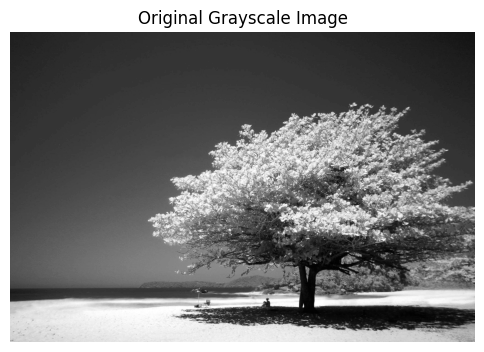
\includegraphics[width=0.5\textwidth]{Images/image.png}
        \caption{Image generated}\label{fig:image}
    \end{figure}

    \subsection{Question 18}

    In order to encode a grayscale image using a fixed-length binary code,
    we must determine the minimum number of bits required to represent all possible 
    pixel intensity values.\\

    \noindent
    A grayscale image typically represent pixel intensities as integer values 
    ranging from:
    \begin{align*}
        \text{Minimum } 0 \text{ to Maximum } 255
    \end{align*}

    \noindent
    So there is 256 distinct values.\\

    \noindent
    To represent 256 distinct values in binary, we must choose the smallest integer $b$ such that:
    \begin{align*}
        2^b \geq 256
    \end{align*}

    \noindent
    Solving this gives:
    \begin{align*}
        b = \lceil \log_2(256) \rceil = \lceil 8 \rceil = 8 \text{ bits}
    \end{align*}

    \noindent
    This matches the required range [0,255] perfectly. 
    Any representation using fewer than 8 bits (e.g., 7 bits → 128 values) 
    would be insufficient to encode the full grayscale spectrum, leading to 
    a loss of information and reduced image quality.

    \subsection{Question 19}

    In our simulation, we modeled the transmission of a grayscale image through a noisy channel 
    using a Binary Symmetric Channel (BSC) with a crossover probability $p=0.01$. 
    This means that each bit of the transmitted image has a 1\% chance of being flipped 
    (from 0 to 1 or vice versa) independently of the others.\\

    \noindent
    The resulting image (see figure \ref{fig:image_bsc}), after transmission through the BSC, exhibits noticeable noise artifacts:
    \begin{figure}[ht]
        \centering
        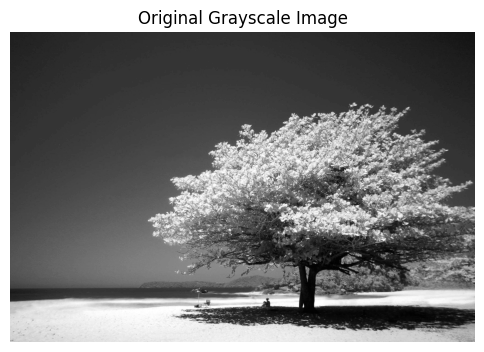
\includegraphics[width=0.4\textwidth]{Images/image.png}
        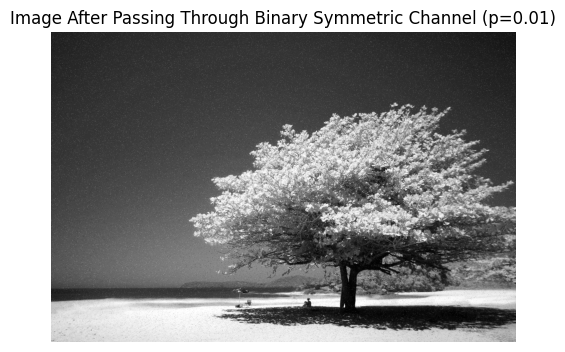
\includegraphics[width=0.5\textwidth]{Images/image_bsc.png} 
        \caption{Image after transmission through the BSC}\label{fig:image_bsc}
    \end{figure}

    \noindent
    The noise introduced by the channel manifests as random speckling and abrupt variations in pixel intensity across the image. 
    As a result, edges become less defined and fine structural details are partially lost or distorted. 
    Overall, the image exhibits a noticeable reduction in clarity and visual fidelity when compared to the original.

    \subsection{Question 20}

    The resulting image after adding some redundancy and passing through the BSC is shown in figure \ref{fig:image_bsc_redundancy}.
    \begin{figure}[ht]
        \centering
        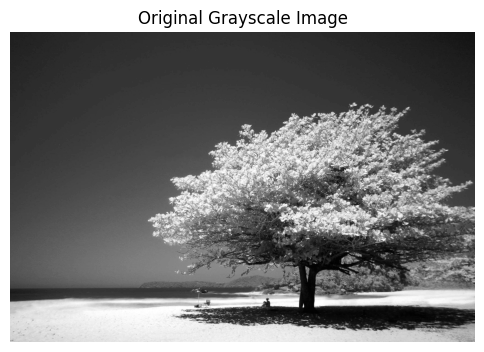
\includegraphics[width=0.4\textwidth]{Images/image.png}
        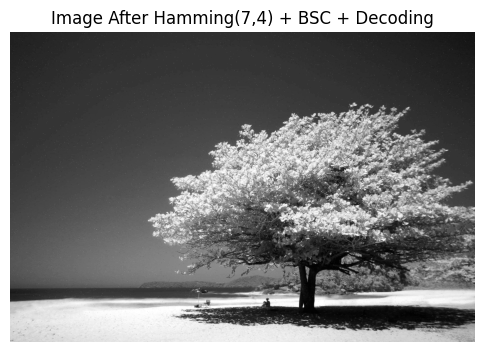
\includegraphics[width=0.5\textwidth]{Images/image_bsc_redundancy.png} 
        \caption{Image after adding some redundancy and passing through the BSC}\label{fig:image_bsc_redundancy}
    \end{figure}

    \noindent
    The noise noticed in this image is less visible than for the previous image.
    This improvement is due to the Hamming code's ability to identify and correct 
    single-bit errors, which are the most likely type of corruption under the given channel conditions. 
    Although this approach increases the data size by a factor of $\frac{7}{4}$, the trade-off is 
    justified by the substantial gain in visual quality and robustness.  

    \subsection{Question 21}

    \subsection{Question 22}

\end{document}
